%\documentclass[handout]{beamer}
\documentclass{beamer}
\usepackage{amsmath}
\usepackage{stdpresent}
%\usepackage[margin=1in]{geometry}
\usepackage{tikz}
\usepackage{natbib}
\usepackage{booktabs}
\usepackage{verbatim}
\usepackage{tikz}
\usetikzlibrary{intersections,positioning}
\usetikzlibrary{matrix, calc}
\newcommand*{\hnode}[1]{\node[outer sep=0pt,anchor=base] (#1) {#1};} 
\usepackage[absolute,overlay]{textpos}
\usetikzlibrary{bayesnet}
\usepackage{tcolorbox}
\usepackage{subfigure}
\usepackage{stackengine}
\usepackage{vimacros}


%\usepackage{subcaption}
\usepackage[tikz]{bclogo}


\newcommand{\cblue}[1]{\textcolor{blue}{{#1}}}
\newcommand{\cred}[1]{\textcolor{red}{{#1}}}

\title[DGM4NLP]{Deep Generative Language Models}
\subtitle{DGM4NLP}

\def\W#1#2{\rnode{#1}{#2}\hfill}

\newcommand{\pointthis}[2]{
        \tikz[remember picture,baseline]{\node[anchor=base,inner sep=0,outer sep=0]%
        (#1) {\textbf{#1}};\node[overlay,rectangle callout,%
        callout relative pointer={(0.1cm,0.5cm)},fill=yellow!90] at ($(#1.north)+(-.5cm,-1cm)$) {#2};}%
        }%

\newcommand{\ack}[1]{\let\thefootnote\relax\footnote{\textcolor{gray}{#1}}}

\presetkeys{bclogo}{
ombre=true,
epBord=3,
couleur = blue!15!white,
couleurBord = red,
arrondi = 0.2,
logo=\bctrombone
}{}

\author[Rios]{Miguel Rios\\University of Amsterdam}
\date{\today}

% add page num
\expandafter\def\expandafter\insertshorttitle\expandafter{%
  \insertshorttitle\hfill%
  \insertframenumber\,/\,\inserttotalframenumber}

\begin{document}
\maketitlepage


\section{Language Modelling}

\frame{ \frametitle{Recap Generative Models of Word Representation}
\begin{textblock*}{\textwidth}(0.1\textwidth,0.25\textheight)
\center Discriminative embedding models\\ \textbf{word2vec} 
\end{textblock*}

\begin{textblock*}{\textwidth}(0.1\textwidth,0.4\textheight)
	\begin{small}
	\begin{center}
	%\only<1>{
	%\emph{\textcolor{blue}{In the event of a chemical spill,} \textcolor{blue}{most children know they should} {\bf evacuate} \textcolor{blue}{as advised by people in} \textcolor{blue}{charge.}}}
	%\only<2-4>{
	\emph{\textcolor{red}{In the event of a chemical spill,} \textcolor{blue}{most children know they should} {\bf evacuate} \textcolor{blue}{as advised by people in} \textcolor{red}{charge.}}
	%}
	%\only<5->{
	%\emph{\textcolor{red}{In the event of a chemical spill,} \textcolor{blue}{most children know they should} \pointthis{evacuate}{ambiguity} \textcolor{blue}{as advised by people in} \textcolor{red}{charge.}}}
	\end{center}
	\end{small}
	\end{textblock*}
	
	
	\begin{textblock*}{\textwidth}(0.2\textwidth,0.6\textheight)
	
	\only<1->{
	Place words in $\mathbb R^d$ as to answer questions like

	\begin{center}	
	\emph{``Have I seen this word in this context?''}
	\end{center}
	}
	
	\only<2->{
	Fit a binary classifier
	\begin{itemize}
		\item \textcolor{blue}{positive} examples
		\item \alert{negative} examples\\ 		
	\end{itemize}
	}
	\end{textblock*}

}

\frame{ \frametitle{Recap Generative Models of Word Representation}
\begin{itemize}

\item The models processes a sentence and outputs a word representation:
\begin{figure}
	\includegraphics[scale=0.40]{elmo-bert-gpt}
\end{figure}


\end{itemize}

}





\frame{ \frametitle{Recap Generative Models of Word Representation}


	\begin{textblock*}{\textwidth}(0.21\textwidth,0.23\textheight)
	\begin{center}
		\textcolor{blue}{quickly evacuate the area} ~ / ~  \textcolor{orange!90!yellow}{deje el lugar r\'{a}pidamente}
	\end{center}
	\end{textblock*}
	
	\begin{textblock*}{0.3\textwidth}(0.025\textwidth,0.35\textheight)
	\scalebox{0.7}{
	%\begin{figure}
%\center
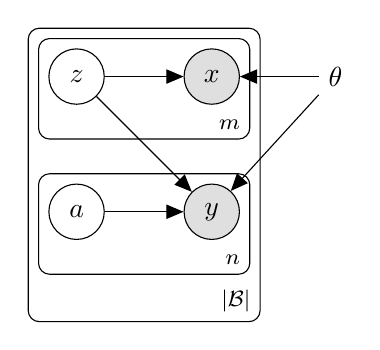
\begin{tikzpicture}
\node[obs]	                   (x)		{$ x $};
\node[obs, below = of x]	       (y)		{$ y $};
\node[latent, left = of x]		(z)		{$ z $};
\node[latent, left = of y]		(a)		{$ a $};
\node[right = of x] (theta) {$\theta$};

% Connect nodes
\edge{a}{y};
\edge{z}{x};
\edge{z}{y};
\edge{theta}{y,x};

% add plates
\plate {L1-sentence} {(x)(z)} {$ m $};
\plate {L2-sentence} {(y)(a)} {$ n $};
\plate {corpus} {(L1-sentence) (L2-sentence)} {$|\mathcal B|$};

\end{tikzpicture}
%\caption{\label{fig:GM2}This model is a refinement of that in \rfig{GM1}, where the latent variable $z$ that participates in generating the aligned sentences. This allows for representations to be ``disambiguated'' in context.}
%\end{figure}
	}
	\end{textblock*}
	
	\begin{textblock*}{\textwidth}(0.32\textwidth,0.35\textheight)
	\begin{figure}
    \begin{overprint}
    \onslide<1>\includegraphics[scale=0.2]{animation/embed1}
    \onslide<2>\includegraphics[scale=0.2]{animation/embed2}
    \onslide<3>\includegraphics[scale=0.2]{animation/embed3}
    \onslide<4>\includegraphics[scale=0.2]{animation/embed4}
    \onslide<5>\includegraphics[scale=0.2]{animation/embed5}
    \onslide<6>\includegraphics[scale=0.2]{animation/embed6}
    \onslide<7>\includegraphics[scale=0.2]{animation/embed7}
    \onslide<8>\includegraphics[scale=0.2]{animation/embed8}
    \onslide<9->\includegraphics[scale=0.2]{animation/embed9} 
    \end{overprint}
\end{figure}
	%\includegraphics[scale=0.2]{animation/embed1}
	%\includegraphics[scale=0.2]{animation/embed2} \pause
	%\includegraphics[scale=0.2]{animation/embed3} \pause
	%\includegraphics[scale=0.2]{animation/embed4} \pause
	%\includegraphics[scale=0.2]{animation/embed5} \pause
	%\includegraphics[scale=0.2]{animation/embed6} \pause
	%\includegraphics[scale=0.2]{animation/embed7} \pause
	%\includegraphics[scale=0.2]{animation/embed8} \pause
	%\includegraphics[scale=0.2]{animation/embed9} \pause
	
	%\begin{small}
	%		\begin{tabular}{p{0.5cm} | p{1.5cm} p{1.5cm} p{1.5cm} p{1.5cm}}
	%		\only<3->{$X$ & \textcolor{blue}{quickly$_1$} & \textcolor{blue}{evacuate$_2$} & \textcolor{blue}{the$_3$} & \textcolor{blue}{area$_4$}} \\
	%		\only<3->{& $\uparrow$ & $\uparrow$ & $\uparrow$ & $\uparrow$} \\
	%		\only<2->{$Z$ & $z_{\textcolor{blue}{1}}$ & $z_{\textcolor{blue}{2}}$ & $z_{\textcolor{blue}{3}}$ & $z_{\textcolor{blue}{4}}$} \\
	%		& & & & \\
	%		\only<4->{$A$ & $a_{\textcolor{orange!90!yellow}{1}}=\textcolor{blue}{2}$ & $a_{\textcolor{orange!90!yellow}{2}}=\textcolor{blue}{3}$ & $a_{\textcolor{orange!90!yellow}{3}}=\textcolor{blue}{4}$ & $a_{\textcolor{orange!90!yellow}{4}}=\textcolor{blue}{1}$ }\\
	%		\only<5->{$Z_a$ & $z_{\textcolor{blue}{2}}$ & $z_{\textcolor{blue}{3}}$ & $z_{\textcolor{blue}{4}}$ & $z_{\textcolor{blue}{1}}$} \\
	%		 \only<6->{& $\downarrow$ & $\downarrow$ & $\downarrow$ & $\downarrow$ } \\
	%		\only<6->{$Y$ & \textcolor{orange!90!yellow}{deje$_1$} & \textcolor{orange!90!yellow}{el$_2$} & \textcolor{orange!90!yellow}{lugar$_3$} & \textcolor{orange!90!yellow}{r\'{a}pidamente$_4$}} \\
		%	\end{tabular}
	%\end{small}
	\end{textblock*}
	
	%\begin{textblock*}{\textwidth}(0.1\textwidth,0.9\textheight)
	%Marginalising alignments collects additional training data for $z$
	%\end{textblock*}


}

\frame[<+->]{ \frametitle{Recap Generative Models of Word Representation}
%\begin{textblock*}{0.35\textwidth}(0.8\textwidth,0.05\textheight)

\begin{figure}
  \includegraphics[width=0.42\textwidth]{architecture.pdf}
 %  \hfill
%   \includegraphics[width=0.42\textwidth]{dec.png}
\end{figure}


%\end{textblock*}

%\begin{textblock*}{\textwidth}(0.05\textwidth,0.15\textheight)
%\begin{itemize}
%\item Embedding 128d
%\item BiLSTM 128d
%\item Z 100d
%\end{itemize}
%\end{textblock*}
}



\frame[<+->]{ \frametitle{Introduction}
\begin{itemize}
\item  you know nothing, jon \cblue{x}
\item ground control to major \cblue{x}
\item the \cblue{x}

\end{itemize}

}

\frame[<+->]{ \frametitle{Introduction}
\begin{itemize}
\item  the quick brown \cblue{x}
\item  the quick brown  fox \cblue{x}
\item  the quick brown  fox  jumps \cblue{x}
\item  the quick brown  fox  jumps  over \cblue{x}
\item  the quick brown  fox  jumps over the  \cblue{x}
\item  the quick brown  fox  jumps  over the lazy \cblue{x}
\item  the quick brown  fox  jumps over the lazy dog 
\end{itemize}

}

\frame[<+->]{ \frametitle{Definition}
\begin{itemize}
\item Language models give us the probability of a sentence;
\item At a time step, they assign a probability to the next word.
\end{itemize}
}



\frame[<+->]{ \frametitle{Applications}
\begin{itemize}
\item Very useful on different tasks:
\item Speech recognition;
\item Spelling correction;
\item Machine translation;

\item  LMs are useful in almost any tasks that deals with generating language.
\end{itemize}
}

\frame[<+->]{ \frametitle{Language Models}
\begin{itemize}
\item N-gram based LMs;
\item  Log-linear LMs;
\item  Neural LMs.
\end{itemize}
}

\frame[<+->]{ \frametitle{N-gram LM}
\footnotesize{
\begin{itemize}
\item $x$ is a sequence of words 
\item $x = {x_1, x_2, x_3, x_4, x_5}$ \\
= {you, know, nothing, jon, snow}
\end{itemize}
}
}

\frame[<+->]{ \frametitle{N-gram LM}

\begin{itemize}
\item To compute the probability of a sentence \\
\begin{equation}
p(x)=p\left(x_{1}, x_{2}, \ldots, x_{n}\right)
\end{equation}
\item We apply the chain rule: \\
\begin{equation}
p(x)=\prod_{i} p\left(x_{i} | x_{1}, \ldots, x_{i-1}\right)
\end{equation}
\item We limit the history with a Markov order: \\

$p\left(x_{i} | x_{1}, \ldots, x_{i-1}\right) \simeq p\left(x_{i} | x_{i-4}, x_{i-3}, x_{i-2}, x_{i-1}\right)$


\end{itemize}
\ack{\citep{JelMer80, Goodman:2001:BPL:2791595.2791976}}
}


\frame[<+->]{ \frametitle{N-gram LM}

\begin{itemize}

\item Chain rule:
\begin{equation}
p(x)=\prod_{i} p\left(x_{i} | x_{1}, \ldots, x_{i-1}\right)
\end{equation}
\item 
\begin{figure}
	\includegraphics[scale=0.40]{markov}
\end{figure}

\end{itemize}

}


\frame[<+->]{ \frametitle{N-gram LM}

\begin{itemize}

\item We make a Markov assumption of conditional independence:
\begin{equation}
p\left(x_{i} | x_{1}, \ldots, x_{i-1}\right) \simeq p\left(x_{i} | x_{i-1}\right)
\end{equation}
\item 
\begin{figure}
	\includegraphics[scale=0.50]{chainrule}
\end{figure}

\end{itemize}

}


\frame[<+->]{ \frametitle{N-gram LM}

\begin{itemize}

\item We make the Markov assumption:\\

$p\left(x_{i} | x_{1}, \ldots, x_{i-1}\right) \simeq p\left(x_{i} | x_{i-1}\right)$
\item If we do not observe the bigram $p(x_i| x_{i-1})$ is 0 \\
and the probability of a sentence will be 0.
\item MLE
\begin{equation}
p_{\mathrm{MLE}}\left(x_{i} | x_{i-1}\right)=\frac{\operatorname{count}\left(x_{i-1}, x_{i}\right)}{\operatorname{count}\left(x_{i-1}\right)}
\end{equation}
\item Laplace smoothing:
\begin{equation}
p_{\mathrm{add}1}\left(x_{i} | x_{i-1}\right)=\frac{\operatorname{count}\left(x_{i-1}, x_{i}\right)+1}{\operatorname{count}\left(x_{i-1}\right)+V}
\end{equation}
\end{itemize}

}


\frame[<+->]{ \frametitle{Log-linear LM}

\begin{itemize}

\item 
\begin{equation}
p(y | x)=\frac{\exp \boldsymbol{w} \cdot \phi(x, y)}{\sum_{y^{\prime} \in V_{y}} \exp w \cdot \phi\left(x, y^{\prime}\right)}
\end{equation}
\item $y$ is the next word and $V_y$ is the vocabulary;
\item $x$ is the history;
\item $\phi$ is a feature function that returns an n-dimensional vector;
\item $w$ are the model parameters.
\end{itemize}

}


\frame[<+->]{ \frametitle{Log-linear LM}

\begin{itemize}

\item n-gram features $x_{j-1}$ =  the and $x_j$ = puppy.
\item gappy n-gram features $x_{j-2}$ =  the and $x_j$ = puppy.
\item class features: $x_j$  belongs to class ABC;
\item gazetteer features: $x_j$ is a place name;

\end{itemize}

}

\frame[<+->]{ \frametitle{Log-linear LM}

\begin{itemize}

\item With features of words and histories we can share statistical weight
\item With n-grams, there is no sharing at all
\item We also get smoothing for free
\item We can add arbitrary features
\item We use Stochastic Gradient Descent (SGD)
\end{itemize}

}






\frame[<+->]{ \frametitle{Neural LM}

\begin{itemize}

\item n-gram language models have proven to be effective in various tasks
\item log-linear models allow us to share weights through features
\item maybe our history is still too limited, e.g. n-1 words
\item we need to find useful features
\end{itemize}

}


\frame[<+->]{ \frametitle{Feed-forward NLM}

\begin{itemize}

\item With NN we can exploit distributed representations to allow for statistical weight sharing.
\item How does it work:
\begin{enumerate}
\item each word is mapped to an embedding: an m-dimensional feature
vector;
\item a probability function over word sequences is expressed in terms of
these vectors;
\item we jointly learn the feature vectors and the parameters of the
probability function.
\end{enumerate}


\end{itemize}
\ack{\citep{journals/jmlr/BengioDVJ03}}
}

\frame[<+->]{ \frametitle{Feed-forward NLM}

\begin{itemize}

\item Similar words are expected to have similar feature vectors:
(dog,cat), (running,walking), (bedroom,room)
\item With this, probability mass is naturally transferred from (1) to (2):
\item The cat is walking in the bedroom.
\item The dog is running in the room.
\item Take-away message: \\
The presence of only one sentence in the training data will increase
the probability of a combinatorial number of neighbours in sentence
space.


\end{itemize}

}

\frame[<+->]{ \frametitle{Feed-forward NLM}

\begin{itemize}

\item FF-LM \\
 \begin{figure}
	\includegraphics[scale=0.40]{fflm}
\end{figure}
\item $\boldsymbol{E}_{\mathrm{you}}, \boldsymbol{E}_{\mathrm{know}}, \boldsymbol{E}_{\mathrm{nothing}} \in \mathbb{R}^{100}$ \\
\begin{equation}
\begin{array}{l}{\boldsymbol{x}=\left[\boldsymbol{E}_{\mathrm{you}} ; \boldsymbol{E}_{\mathrm{know}} ; \boldsymbol{E}_{\mathrm{nothing}}\right] \in \mathbb{R}^{300}} \\ {\boldsymbol{y}=\boldsymbol{W}_{3} \tanh \left(\boldsymbol{W}_{1} \boldsymbol{x}+\boldsymbol{b}_{1}\right)+\boldsymbol{W}_{2} \boldsymbol{x}+\boldsymbol{b}_{2}}\end{array}
\end{equation}


\end{itemize}

}

\frame[<+->]{ \frametitle{Feed-forward NLM}

\begin{itemize}

\item FF-LM \\
	\begin{figure}
	\includegraphics[scale=0.40]{fflm}
\end{figure}
\item The non-linear activation functions perform feature combinations that a linear model cannot do;
\item  End-to-end training on next word prediction.

\end{itemize}

}

\frame[<+->]{ \frametitle{Feed-forward NLM}

\begin{itemize}

\item  FF-LM \\
	\begin{figure}
	\includegraphics[scale=0.40]{fflm}
\end{figure}
\item We now have much better generalisation, but still a limited history/context.
\item Recurrent neural networks have unlimited history

\end{itemize}

}

\frame[<+->]{ \frametitle{Feed-forward NLM}

\begin{itemize}

\item FF-LM \\
\begin{figure}
	\includegraphics[scale=0.25]{ffnn-lm}
\end{figure}
\item We now have much better generalisation, but still a limited history/context.
\item Recurrent neural networks have unlimited history

\end{itemize}

}

\frame[<+->]{ \frametitle{RNN NLM}

\begin{itemize}

\item RNN-LM \\
\begin{figure}
	\includegraphics[scale=0.20]{rnnlm}
\end{figure}
\item Start: predict second word from first

\end{itemize}
\ack{\citep{conf/interspeech/MikolovKBCK10}}
}


\frame[<+->]{ \frametitle{RNN NLM}

\begin{figure}
	\includegraphics[scale=0.20]{rnn-lm}
\end{figure}



}





\section{Variational Auto-encoder for Sentences}


\frame[<+->]{ \frametitle{Sen VAE}

\begin{itemize}

\item Model observations as draws from the marginal of a DGM. 
\item An NN maps from a latent sentence embedding $z \in R^{dz}$  to a distribution $p(x|z, \theta)$ over sentences,
\begin{equation}
\begin{array}{l}{p(x | \theta)=\int p(z) p(x | z, \theta) \mathrm{d} z} \\ {=\int \mathcal{N}(z | 0, I) \prod_{i=1}^{|x|} \operatorname{Cat}\left(x_{i} | f\left(z, x_{<i} ; \theta\right)\right) \mathrm{d} z}\end{array}
\end{equation}
\end{itemize}

\ack{\citep{DBLP:journals/corr/BowmanVVDJB15}}
}

\begin{frame}{Sen VAE}
	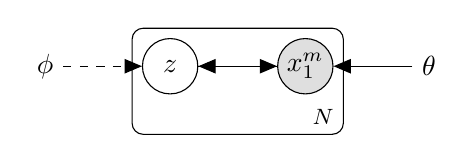
\begin{tikzpicture}
    % Define nodes
    \node[latent]		(z)		{$ z $};
    \node[obs, right = of z]		(x)		{$ x_1^m $};
    \node[right = of x]		(theta)		{$ \theta $};
    
    % Connect nodes
    \edge{z,theta}{x};
    
    % add plates
    \plate {x-sentence} {(x)(z)} {$ N $};
   
    \node[left = of z]		(lambda)		{$\phi $};   
    \edge[dashed, bend right]{x}{z};
    \edge[dashed]{lambda}{z};
    \end{tikzpicture}

	Generative model
    	\begin{itemize}
			\item $Z \sim \mathcal N(0, I)$
			\item $X_i | z, x_{<i} \sim \Cat(f_\theta(z, x_{<i}))$\\
			%where $x_{<i}$ is represented by a recurrent hidden state\\
			%and the categorical parameters are predicted by a single hidden layer FFNN with softmax activation
    	\end{itemize}
	Inference model
    	\begin{itemize}
			\item $Z \sim \mathcal N(\mu_\phi(x_1^m), \sigma_\phi(x_1^m)^2)$
			%where $x_1^m$ is represented by the average embedding\\
			%location and scale are single hidden layer FFNNs
    	\end{itemize}
	
	
	
\end{frame}


\frame[<+->]{ \frametitle{Sen VAE}

\begin{itemize}
 
 \item Generation is one word at a time without Markov assumptions, but $f()$conditions on $z$ \\
 in addition to the observed prefix.
 \item  The conditional $p(x|z, \theta)$ is the decoder.
 \item $p(x | \theta)$ is the marginal likelihood.
 \item We train the model  to assign high (marginal) probability to observations like a  LMs. 
 \item However the model uses a latent space  to exploit neighbourhood and smoothness in latent
space to capture regularities in data space.\\
 For example, it may group sentences according to certain e.g. lexical choices, syntactic complexity, lexical semantics, etc...
 
\end{itemize}
}




\frame[<+->]{ \frametitle{Approximate Inference}

\begin{itemize}
\item The model has  a diagonal Gaussian distribution as variational posterior: \\
$q_{\phi}(z | x)=\mathcal{N}\left(z | \mu_{\phi}(x), \operatorname{diag}\left(\sigma_{\phi}(x)\right)\right)$
\item With reparametrisation:
$z=h_{\phi}(\epsilon, x)=\mu_{\phi}(x)+\sigma_{\phi}(x) \odot \epsilon, \quad \text { where } \epsilon \sim \mathcal{N}\left(0, \mathbf{I}\right)f$
\item Analytical KL: \\
$\mathrm{KL}\left[q_{\phi}(z | x) \| p_{\theta}(z)\right]=\frac{1}{2} \sum_{d=1}^{\mathrm{D}_{z}}\left(-\log \sigma_{\phi}^{2}(x)-1+\sigma_{\phi}^{2}(x)+\mu_{\phi}^{2}(x)\right)$
\end{itemize}
}


\frame[<+->]{ \frametitle{Approximate Inference}

\begin{itemize}
\item We jointly estimate the parameters of both generative and inference by maximising a lowerbound on
the log-likelihood function (ELBO):
\begin{equation}
\begin{array}{r}{\mathcal{L}(\theta, \phi | x)= \mathbb{E}_{q(z | x, \phi)}[\log p(x | z, \theta)].} \\ {-\operatorname{KL}(q(z | x , \phi ) | p(z)) }\end{array}
\end{equation}
\end{itemize}
}


\frame[<+->]{ \frametitle{Architecture}
\begin{itemize}
\item Gaussian Sen VAE  parametrises a categorical distribution over the vocabulary for each given prefix, and, it conditions on a latent embedding:\\
$Z \sim \mathcal{N}(0, I),$ \\ $ \quad X_{i} | z, x_{<i} \sim \operatorname{Cat}\left(f\left(z, x_{<i} ; \theta\right)\right)$
\item 
\begin{equation}
\begin{aligned} 
f\left(z, x_{<i} ; \theta\right) &=\operatorname{softmax}\left(\mathbf{s}_{i}\right) \\
\mathbf{e}_{i} &=\operatorname{emb}\left(x_{i} ; \theta_{\mathrm{emb}}\right) \\ \mathbf{h}_{0} &=\tanh \left(\operatorname{affine}\left(z ; \theta_{\text { init }}\right)\right) \\ \mathbf{h}_{i} &=\operatorname{GRU}\left(\mathbf{h}_{i-1}, \mathbf{e}_{i-1} ; \theta_{\mathrm{gru}}\right) \\ \mathbf{s}_{i} &=\operatorname{affine}\left(\mathbf{h}_{i} ; \theta_{\mathrm{out}}\right) \end{aligned}
\end{equation}
\end{itemize}
}


\frame[<+->]{ \frametitle{ The Strong Decoder Problem}
\begin{itemize}
\item The VAE may ignore the latent variable given the interaction between the prior and posterior in the KL divergence.
\item  This problem appears when we have strong decoders  conditional likelihoods $p(x|z)$ 
parametrised by high capacity models
\item The model might achieve a high ELBO without using information from $z$
\item RNN LM is strong decoder because they condition on all previous context when generating a word
\end{itemize}
}

%\frame[<+->]{ \frametitle{An Information-Theoretic Perspective}

%}

\frame[<+->]{ \frametitle{What to do?}
\begin{itemize}
\item Weakening the Decoder, the model relies on the latent variables the reconstruction of the observed data.
\item KL Annealing, weigh the KL term in the ELBO with a factor that is annealed from 0 to 1 over a fixed number of steps of size $\gamma \in (0, 1)$
\item Word Dropout, by dropping a percentage of the input at random, the decoder has to rely on the latent variable to fill in the missing gaps. 
\item Freebits  because it allows encoding the
first $r$ nats of information for free.\\
$\max (r, \operatorname{KL}(q_{\phi}(z | x) \| p(z)))$
\end{itemize}
}

\frame[<+->]{ \frametitle{Metrics}
\begin{itemize}
\item For VAE models, Negative log-likelihood NLL is estimated, since we do not have access to
the exact marginal likelihood. 
\item We use an importance sampling (IS) estimate://
\begin{equation}
\begin{array}{l}{p(x | \theta)=\int p(z, x | \theta) \mathrm{d} z \stackrel{\mathrm{IS}}{=} \int q(z | x) \frac{p(z, x | \theta)}{q(z | x)} \mathrm{d} z} \\ {\approx \frac{1}{S} \sum_{s=1}^{S} \frac{p\left(z^{(s)}, x | \theta\right)}{q\left(z^{(s)} | x\right)} \text { where } z^{(s)} \sim q(z | x)}\end{array}
\end{equation}
\item Perplexity PPL:  the exponent of average per-word
entropy, given $N$ i.i.d. sequences \\
\begin{equation}
\operatorname{PPL}=\exp \left(\frac{\sum_{i=1}^{N} \log p\left(x_{i}\right)}{\sum_{i=1}^{N}\left|x_{i}\right|}\right)
\end{equation}
\item perplexity is based on the importance sampled NLL

\end{itemize}
}


\frame[<+->]{ \frametitle{Baseline}
\begin{itemize}
\item  RNNLM (Dyer et al., 2016)
\item At each step, an RNNLM parameterises a categorical distribution over the vocabulary, i.e. \\
  $X_{i} | x_{<i} \sim \operatorname{Cat}\left(f\left(x_{<i} ; \theta\right)\right)$ and
 \begin{equation}
 \begin{aligned} 
 f\left(x_{<i} ; \theta\right)=& \operatorname{softmax}\left(\mathbf{s}_{i}\right) \text { and } \\ \mathbf{e}_{i} &=\operatorname{emb}\left(x_{i} ; \theta_{\mathrm{emb}}\right) \\ \mathbf{h}_{i} &=\operatorname{GRU}\left(\mathbf{h}_{i-1}, \mathbf{e}_{i-1} ; \theta_{\mathrm{gru}}\right) \\ \mathbf{s}_{i} &=\operatorname{affine}\left(\mathbf{h}_{i} ; \theta_{\mathrm{out}}\right)
  \end{aligned}
 \end{equation}
 \item  Embedding layer (emb), one (or more) GRU cell(s) ($h_0 \in \theta$ is a parameter of the
model), and an affine layer to map from the dimensionality of the GRU to the vocabulary size.
\end{itemize}
}


\frame[<+->]{ \frametitle{Data}
\begin{itemize}
\item Wall Street Journal part of the Penn Treebank corpus
\item Preprocessing on train-validation-test split as \citep{dyer-etal-2016-recurrent}
\item  WSJ section 1-21 training,
\item  Section 23 as test corpus 
\item Section 24 as validation

\end{itemize}
}


\frame[<+->]{ \frametitle{Results}
\centering
\begin{tabular}{|c|c|c|}
\hline
          & NLL$\downarrow$            & PPL$\downarrow$          \\ \hline
RNN-LM    & 118.7$\pm$0.12 & 107.1$\pm$0.46 \\ \hline
VAE       & 118.4$\pm$0.09 & 105.7$\pm$0.36 \\ \hline
Annealing & 117.9$\pm$0.08 & 103.7$\pm$0.31 \\ \hline
Free-bits & 117.5$\pm$0.18 & 101.9$\pm$0.77 \\ \hline
\end{tabular}
}


\frame[<+->]{ \frametitle{Samples}
\begin{itemize}
\item decode greedily from a prior sampl and the variability is due to the generator’s reliance on the latent sample.
\item The VAE ignores z and greedy generation from a prior sample is essentially deterministic in that case \\
\begin{figure}
	\includegraphics[scale=0.50]{sample}
\end{figure}
\end{itemize}
}


\frame[<+->]{ \frametitle{Samples}
\begin{itemize}
\item Homotopy, decode greedily from
points lying between a posterior sample conditioned on the first sentence and a posterior sample conditioned on the last sentence.
\begin{figure}
	\includegraphics[scale=0.50]{sample1}
\end{figure}
\end{itemize}
}







\section*{References}
	
	%
\frame[plain]{
	\frametitle{Earley intersection}
	
	\begin{footnotesize}
	\begin{align*}
	\textsc{Axioms} & \\
	& \drule{}{\itembrack{S' \ra \bullet S, q, q}}{q \in I} \\
	\textsc{Goal} & \\
	& \itembrack{S' \ra S \bullet, q, r} ~ q \in I \wedge r \in F\\
	\textsc{Scan} & \\
	& \drule{\itembrack{X \ra \alpha \bullet x \beta, q, s}}{\itembrack{X \ra \alpha x \bullet \beta}}{\angbrack{s, x, r} \in E}\\
	\textsc{Predict} & \\
	& \drule{\itembrack{X \ra \alpha \bullet Y \beta, q, r}}{\itembrack{Y \ra \bullet \gamma, r, r}}{Y \ra \gamma \in R} \\
	\textsc{Complete} & \\
	& \drule{\itembrack{X \ra \alpha \bullet Y \beta, q, s}\itembrack{Y \ra \gamma \bullet, s, r}}{\itembrack{X \ra \alpha Y_{s,r} \bullet \beta, q, r}}{X \neq S'} \\
	\textsc{Accept} & \\
	& \drule{\itembrack{S' \ra \bullet S, q, q}\itembrack{S \ra \gamma \bullet, q, r}}{\itembrack{S' \ra  S_{q,r} \bullet, q, r}}{r \in F} 
	\end{align*}
	\end{footnotesize}

	
}




	\frame[allowframebreaks]{ \frametitle{References}
	
        \bibliographystyle{plainnat}
        \bibliography{BIB}
	}


\end{document}
\grid
